% Number 780
% CAPMA CAPMG Algebra Units 
% Rocket AP problem - graphical and algebraic
% Mostly AP/some JG

% Watermark
\AddToShipoutPicture*{\BackgroundPic}

\addtocounter {ProbNum} {1}

%\begin{floatingfigure}[r]{.44\textwidth}
%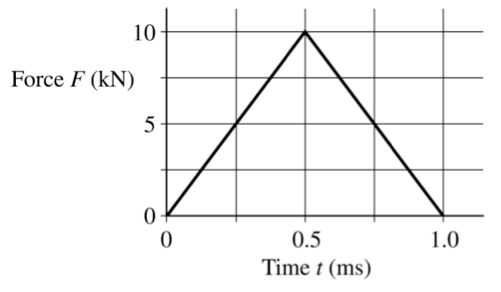
\includegraphics[scale=.5]{/Users/jgates/desktop/latex/pics/collisiongraph1}
%\end{floatingfigure}
 
{\bf \Large{\arabic{ProbNum}}} A two stage rocket leaves its launch pad moving vertically with an average acceleration of ${4~\tfrac{m}{s^2}}$.  10 seconds after launch, the first stage of the rocket (now without fuel) separates from the second stage  The second stage now has an upward acceleration of ${6~\tfrac{m}{s^2}}$.  

\bigskip
How high is the rocket when the first stage separates?

\vfill

What will be the maximum height attained by the first stage after separation?

\vfill

\newpage 
% Watermark
\AddToShipoutPicture*{\BackgroundPic}
Draw position, velocity, and acceleration graphs for the first and second stages' motions {\emph after separation} on the same three sets of axes (that is, have both velocity graph on one set of axes, both position graphs on another, etc.).

\vfill

\vfill

Use the graphs to determine how far apart the stages are 4 seconds after separation.

\vfill
%\hfill 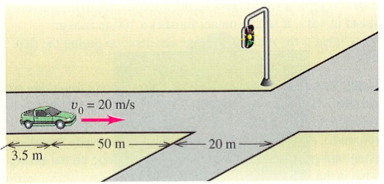
\includegraphics[scale=.85]{/Users/jgates/desktop/latex/pics/redlight.png}
\newpage
